% Section 5 draft: simulations. Numbers are macros from Tabelas/numbers.tex.

\section{Simulations}
\label{sec:simulation}

We use two experiments. The first simulates base forecast errors directly, so that the population error covariance is known and the gain from joint reconciliation can be computed exactly. The second simulates time series, fits base forecasting models, and reconciles their forecasts, as in the original design of this study.

\subsection{Experiment 1: controlled error covariances}

For each of two variables, the base forecast errors are $\bm{e}_j = \bm{S}\bm{u}_j + \bm{v}_j$. The coherent component $\bm{S}\bm{u}_j$ is invisible to reconciliation (Corollary~\ref{cor:invariance}). The incoherent component $\bm{v}_j$ has independent entries across series, with variance $\lambda_{ij}$ for series $i$ and correlation $\rho_i$ between the two variables at series $i$. With this structure, condition (e) of Proposition~\ref{prop:equivalence} holds exactly when $d_i = \rho_i(\lambda_{i2}/\lambda_{i1})^{1/2}$ is the same for every series. We consider five families of covariance matrices, each indexed by a parameter that controls the departure from the conditions of Proposition~\ref{prop:equivalence}. Let $a_i$ be the number of bottom-level series summed by series $i$.
\begin{description}
  \item[F0, separable.] $\lambda_{i1} = \lambda_{i2} = a_i$ and $\rho_i = \rho$, with $\rho$ from $-0.9$ to $0.9$.
  \item[F1, separable plus invisible.] F0 with $\rho = 0.7$, plus a non-separable coherent component $\bm{S}_*\bm{K}\bm{S}_*'$ of increasing size.
  \item[F2, variable-specific profiles.] $\lambda_{i1} = a_i$, $\lambda_{i2} = a_i^{1+\delta}$ and $\rho_i = 0.7$. As $\delta$ grows, the second variable's incoherent errors become increasingly concentrated at the aggregate levels.
  \item[F3, node-varying correlation.] $\lambda_{i1} = \lambda_{i2} = a_i$ and $\rho_i = 0.3 + \delta z_i$, where $z_i \in [-1, 1]$ is a fixed pattern that alternates in sign within each level.
  \item[F4, OLS case.] $\bm{W} = \bm{S}_*\bm{K}\bm{S}_*' + \tau\bm{I}$.
\end{description}
F0, F1 and F4 satisfy Proposition~\ref{prop:equivalence}; F2 and F3 do not when $\delta > 0$. We use two hierarchies: the eight-series hierarchy of Figure~\ref{fig:HTS_M.ex}, and the 33-series hierarchy of the Brazilian application (Section~\ref{sec:application}).

\paragraph{Population results.} Figure~\ref{fig:exp1-gain} shows the exact MSE reduction from joint rather than separate reconciliation, $\gamma(\bm{W})$, against $\kappa(\bm{W})$. For F0, F1 and F4 both are zero to machine precision, whatever the strength of cross-variable correlation, and for F4 joint MinT coincides with OLS reconciliation. For F2 and F3 the gain rises with $\kappa$, but it is modest: at most \gainFtwoBrazilMax\% in the Brazilian hierarchy with $\kappa = \kappaFtwoBrazilMax$, and at most \gainFthreeSmallMax\% for node-varying correlations. Even substantial departures from the conditions of Proposition~\ref{prop:equivalence} buy little accuracy.

\begin{figure}[!htb]
  \centering
  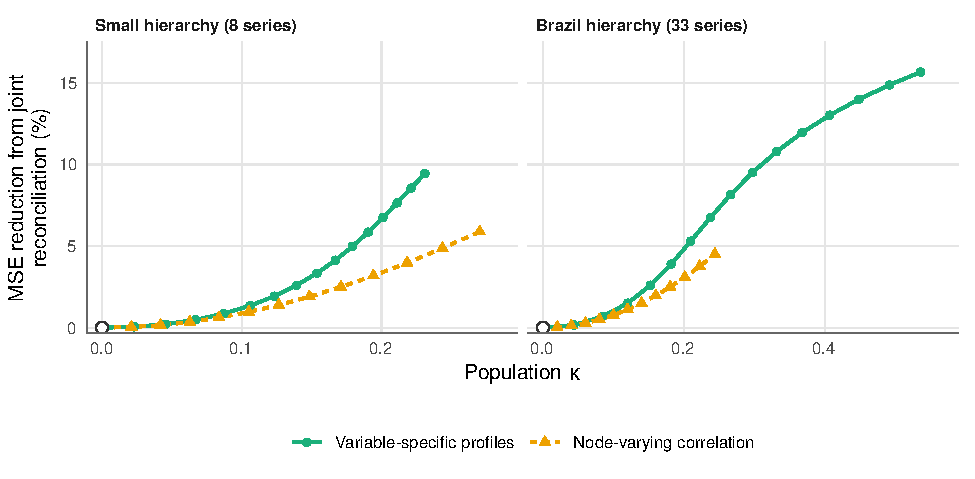
\includegraphics[width=\textwidth]{Imagens/exp1_gain.pdf}
  \caption{Experiment 1: population MSE reduction from joint rather than separate reconciliation against $\kappa$. The separable (F0), separable-plus-invisible (F1) and OLS (F4) families all lie at the origin.}
  \label{fig:exp1-gain}
\end{figure}

\paragraph{Estimated covariances.} In practice $\bm{W}$ is estimated, and the joint estimate has $m^2 = 4$ times as many entries as each separate one. For each family and hierarchy we drew $T \in \{50, 100, 200, 500, 1000, 2000\}$ error vectors from $N(\bm{0}, \bm{W})$, estimated the covariance by shrinkage \eqref{eq:shrink}, and computed the exact expected loss $\operatorname{tr}(\widehat{\bm{M}}\bm{W}\widehat{\bm{M}}')$ of the resulting maps, over \expOneReps{} replications. Figure~\ref{fig:exp1-T} shows the ratio of expected loss for joint to separate reconciliation. Under separability the joint map is never better, and it is worse at small sample sizes: by \sepPenaltySmall\% at $T = 50$ in the small hierarchy and \sepPenaltyBrazil\% in the Brazilian one. That is the price of estimating cross-variable blocks that carry no information. When the population gain is small, the estimated joint map does not recover it until $T$ is in the hundreds or thousands; for the weakest node-varying departure in the Brazilian hierarchy, whose population gain is \gainFthreeWeakBrazil\%, the estimated joint map gains only \gainFthreeWeakBrazilEst\% even at $T = 2000$. Only the largest departures give a clear gain at sample sizes typical of monthly data.

\begin{figure}[!htb]
  \centering
  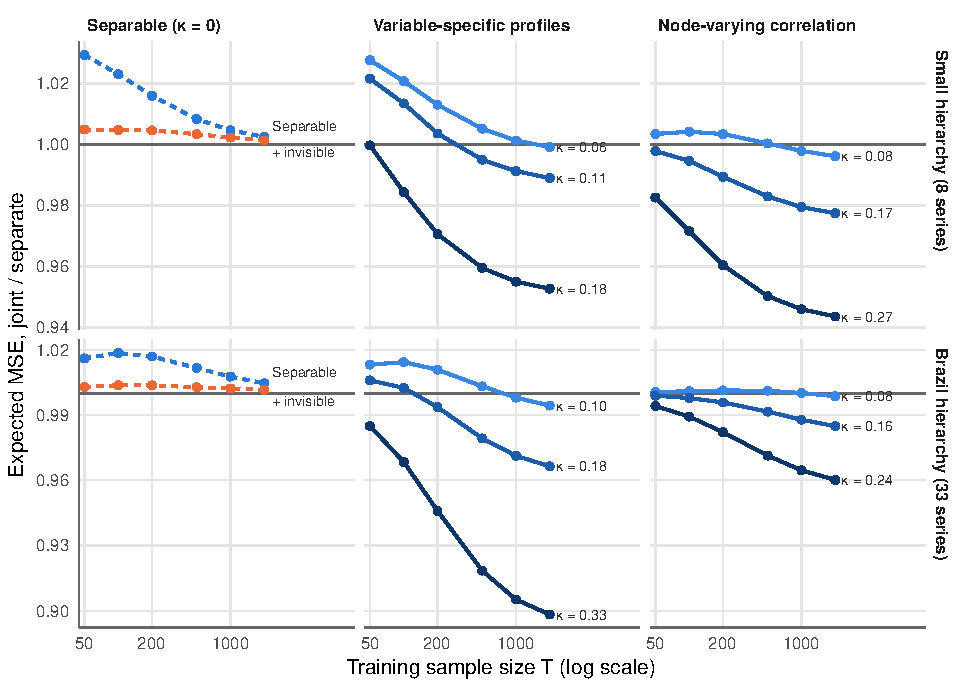
\includegraphics[width=\textwidth]{Imagens/exp1_samplesize.pdf}
  \caption{Experiment 1: expected MSE of joint relative to separate reconciliation with shrinkage estimates of $\bm{W}$, by training sample size. Values below one favour joint reconciliation. Labels give the population $\kappa$.}
  \label{fig:exp1-T}
\end{figure}

\subsection{Experiment 2: fitted base models}

\todo[inline]{Experiment 2: scenarios, population quantities (Table~\ref{tab:exp2}), fitted ARIMA and VAR results. Write after exp2 completes.}
